
Stochastic gradient descent (SGD) is the workhorse algorithm for
optimization in machine learning and stochastic approximation
problems; improving its runtime dependencies is a central issue in
large scale stochastic optimization that often arise in machine 
learning problems at scale~\citep{BottouB07}, where one can only resort to streaming algorithms. 

%Unfortunately, the folklore is that it is not possible to utilize fast gradient methods for stochastic optimization due to their instability and error accumulation.  This work strongly refutes this folklore showing, in very strong sense, that acceleration is robust to \emph{statistical} errors. In particular, we provide an accelerated stochastic gradient descent algorithm that enjoys minimax optimal statistical estimation at rate that is provably faster than stochastic gradient descent.

This work examines these broader runtime issues for the special case of stochastic approximation in the
following least squares regression problem:% (i.e. linear regression) \sidford{Not sure need the i.e. and would get a better line break. Also changed formatting of the 1/2 below}:
\vspace{-0.2cm}
\begin{align}
\label{eq:objFun}
\min_{\x \in \R^d} P(\x), \, \, \, 
\text{where, }P(\x)\defeq \tfrac{1}{2} \cdot\Eover{\distr}{(b-\iprod{\x}{\a})^2},
\end{align}

\vspace{-0.3cm}
\noindent where we have access to a {\em stochastic first order oracle}, which, when provided with $\x$ as an input, returns a noisy unbiased stochastic gradient using a tuple $(\a,\b)$ sampled from $\D(\R^d\times \R)$, with $d$ being the dimension of the problem. A query to the stochastic first-order oracle at $\x$ produces: %an unbiased estimate $\widehat{\nabla}P(\x)$ of the gradient $\nabla P(x)$ of the form 
\vspace{-0.25cm}
\begin{align}
\label{eq:stochFirstOrderOracle}
\widehat{\nabla}P(\x) = \ -(b-\iprod{\a}{\x})\cdot\a.% \quad \text{where, }\E{\widehat{\nabla}P(\x)}=\nabla P(\x)\quad\text{({\em unbiased} estimate)}.
\end{align}
Note $\E{\widehat{\nabla}P(\x)}=\nabla P(\x)$ (i.e. eq\eqref{eq:stochFirstOrderOracle} is an unbiased estimate). Note that nearly all practical stochastic algorithms use sampled gradients of the specific form as in equation~\ref{eq:stochFirstOrderOracle}. We discuss differences to the more general stochastic first order oracle~\citep{NemirovskyY83} in section~\ref{sec:related}.

\begin{table*}[t]
	\begin{center}
  \begin{adjustbox}{max width=\textwidth}
  		\begin{tabular}{| c | c | c | c |}
			\hline
			Algorithm & Final error & Runtime & Memory\\ 
		\hline
			\begin{tabular}{@{}c@{}} Accelerated SVRG \\ \citep{Zhu16} \end{tabular}&  $\mathcal{O}\left(\frac{\sigma^2 d}{n}\right)$ & $({n+\sqrt{n\cnH}})d\log\bigg({\frac{P(\xt[0])-P(\xt[*])}{(\sigma^2d/n)}}\bigg)$ &$nd$\\
			\hline
			\begin{tabular}{@{}c@{}} Streaming SVRG \\ \citep{FrostigGKS15} \\ 	Iterate Averaged SGD \\ \citep{JainKKNS16} \end{tabular} & $\mathcal{O}\left(\exp\left(\frac{-n}{\cnH}\right)\cdot\big(P(\xt[0])-P(\xt[*])\big) + \frac{\sigma^2 d}{n}\right)$ & ${nd}$ &$\mathcal{O}(d)$\\
\hline
			\begin{tabular}{@{}c@{}} Accelerated Stochastic Gradient Descent \\ (this paper) \end{tabular}& $\mathcal{O}^*\left(\exp\left(\frac{-n}{\sqrt{\cnH\cnS}}\right) \big(P(\xt[0])-P(\xt[*])\big)\right) + \mathcal{O}\left(\frac{\sigma^2 d}{n}\right)$ & ${nd}$ &$\mathcal{O}(d)$\\
			\hline
		\end{tabular} 
		\end{adjustbox}
				\caption{Comparison of this work to the best known non-asymptotic results~\citep{FrostigGKS15,JainKKNS16} for the least squares stochastic approximation problem.\iffalse See section~\ref{sec:related} for related work.\fi\ Here, $d,n$ are the problem dimension, number of samples; $\cnH$, $\cnS$ denote the condition number and statistical condition number of the distribution; $\sigma^2$, $P(\xt[0])-P(\xt[*])$ denote the noise level and initial excess risk, $\mathcal{O}^*$ hides lower order terms in $d,\cnH,\cnS$ (see section~\ref{sec:prob} for definitions and a proof for $\cnS \leq \cnH$). Note that Accelerated SVRG~\citep{Zhu16} is not a streaming algorithm. 
                  %For the least squares stochastic approximation problem, there are several
                  %non-asymptotic
                  %analyses~\citep{BachM13,DefossezB15,NeedellSW16,FrostigGKS15,JainKKNS16},
                  %and we refer to the fastest rates in this table. 
                }\vspace*{-1cm}
		\iffalse\caption{Comparison of this work to the best known prior non-asymptotic results~\citep{BachM13,DefossezB15,NeedellSW16,FrostigGKS15,JainKKNS16} for the least squares stochastic approximation problem. Here, $d,n$ are the problem dimension, number of samples;
                  $\cnH$, $\cnS$ denote the condition number and
                  statistical condition number of the distribution,
                  $\sigma^2$ denotes the noise level, and
                  $P(\xt[0])-P(\xt[*])$ denotes the initial excess
                  risk, and $\mathcal{O}^*$ hides lower order terms in
                  $d,\cnH,\cnS$ (see section~\ref{sec:prob} for definitions and a short proof that $\cnS \leq \cnH$). Note that Accelerated SVRG~\citep{Zhu16} is not a streaming algorithm. See section~\ref{sec:related} for related work.
                  %For the least squares stochastic approximation problem, there are several
                  %non-asymptotic
                  %analyses~\citep{BachM13,DefossezB15,NeedellSW16,FrostigGKS15,JainKKNS16},
                  %and we refer to the fastest rates in this table. 
                }\fi
		\label{tab:comp}
	\end{center}
\end{table*}
Let $\xs \eqdef \arg\min_\x P(\x)$ be a population risk minimizer.  Given any estimation procedure which returns $\xhat_n $ using $n$ samples, define the {\em excess risk} (which we also refer to as the \emph{generalization error} or the \emph{error}) of $\xhat_n$ as $\E{P(\xhat_n)}-P(\xs)$.
Now, equipped a stochastic first-order oracle (equation~\eqref{eq:stochFirstOrderOracle}), our goal is to provide a computationally efficient (and streaming) estimation method whose excess risk is comparable to the optimal statistical minimax rate.  

In the limit of large $n$, this minimax rate is achieved by the {\em empirical risk minimizer} (ERM), which is defined as follows. Given $n$ i.i.d. samples $\ST_n=\{(\a_i,\b_i)\}_{i=1}^n$ drawn from $\D$, define 
\vspace*{-3mm}
\begin{align*} 
	\xhat_n^{\textrm{ERM}} \eqdef \arg\min_\x P_n(\x) , \textrm{ where } P_n(\x)\eqdef\frac{1}{n}\sum_{i=1}^{n} \tfrac{1}{2}\left(\b_i-\a_i\T \x \right)^2,
\end{align*}

\vspace{-0.3cm}
\noindent where $\xhat_n^{\textrm{ERM}}$ denotes the ERM over the samples $\ST_n$. For the case of additive noise models (i.e. where $b=\a\T\xs+\n$, with $\n$ being independent of $\a$), the minimax estimation rate is $d\sigma^2/n$~\citep{KushnerClark,PolyakJ92,lehmann1998theory,Vaart00}, i.e.:
\vspace{-0.2cm}
\begin{align} \label{eq:ERMVarianceAdditive}
\lim_{n\to\infty}\frac{\mathbb{E}_{\ST_n}[P(\xhat_n^{\textrm{ERM}})]-P(\xs)}{d\sigma^2/n} &= 1,
\end{align}

\vspace{-0.2cm}
\noindent where $\sigma^2=\E{\n^2}$ is the variance of the additive noise and the expectation is over the samples $\ST_n$ drawn from $\D$.  The seminal works of~\cite{Ruppert88,PolyakJ92} proved that a certain averaged stochastic gradient method enjoys this minimax rate, in the limit.  The question we seek to address is: how fast (in a non-asymptotic sense) can we achieve the minimax rate of $d\sigma^2/n$?\vspace*{-1mm}
\subsection{Review: Acceleration with Exact Gradients}\label{sec:background}
Let us review results in convex optimization in the exact first-order oracle model. Running $t-$steps of gradient descent~\citep{Cauchy1847} with an exact first-order oracle yields the
following guarantee:\vspace*{-2mm}
\begin{align*}
P(\x_t)-P(\xs)\leq \exp\big(-t/\cnH_o\big)\cdot\big(P(\x_0)-P(\xs)\big),
\end{align*}

\vspace{-0.2cm}
\noindent where $\x_0$ is the starting iterate, $\cnH_o=\lambda_{\max}(\H)/\lambda_{\min}(\H)$ is the condition number of $P(.)$, where, $\lambda_{\max}(\H),\lambda_{\min}(\H)$ are the largest and smallest eigenvalue of the hessian $\H=\nabla^2P(\x)=\E{\a\a\T}$. Thus gradient descent requires $\mathcal{O}(\cnH_o)$ oracle calls to solve the problem to a given target accuracy, which is sub-optimal amongst the class of methods with access to an exact first-order oracle~\citep{Nesterov04}. This sub-optimality can be addressed through Nesterov's Accelerated Gradient Descent~\citep{Nesterov83}, which when run for t-steps, yields the following guarantee:
%This sub-optimality is remedied through the {\em accelerated} gradient method~\citep{Nesterov83}, which when run for $t-$steps, yields the following convergence guarantee:
\vspace{-0.2cm}
\begin{align*}
P(\x_t)-P(\xs)\leq \exp\big(-t/\sqrt{\cnH_o}\big)\cdot\big(P(\x_0)-P(\xs)\big),
\end{align*}

\vspace{-0.2cm}
\noindent which implies that $\mathcal{O}(\sqrt{\cnH_o})$ oracle calls are sufficient to achieve a given target accuracy. This matches the oracle lower bounds~\citep{Nesterov04} that state that $\Theta(\sqrt{\cnH_o})$ calls to the exact first order oracle are necessary to achieve a given target accuracy. The conjugate gradient method~\citep{HestenesS52} and heavy ball method~\citep{Polyak64} are also known to obtain this convergence rate for solving a system of linear equations and for quadratic functions. These methods are termed fast gradient methods owing to the improvements offered by these methods over Gradient Descent.
\begin{figure}[t!]
\centering
	\subfigure[Discrete Distribution]{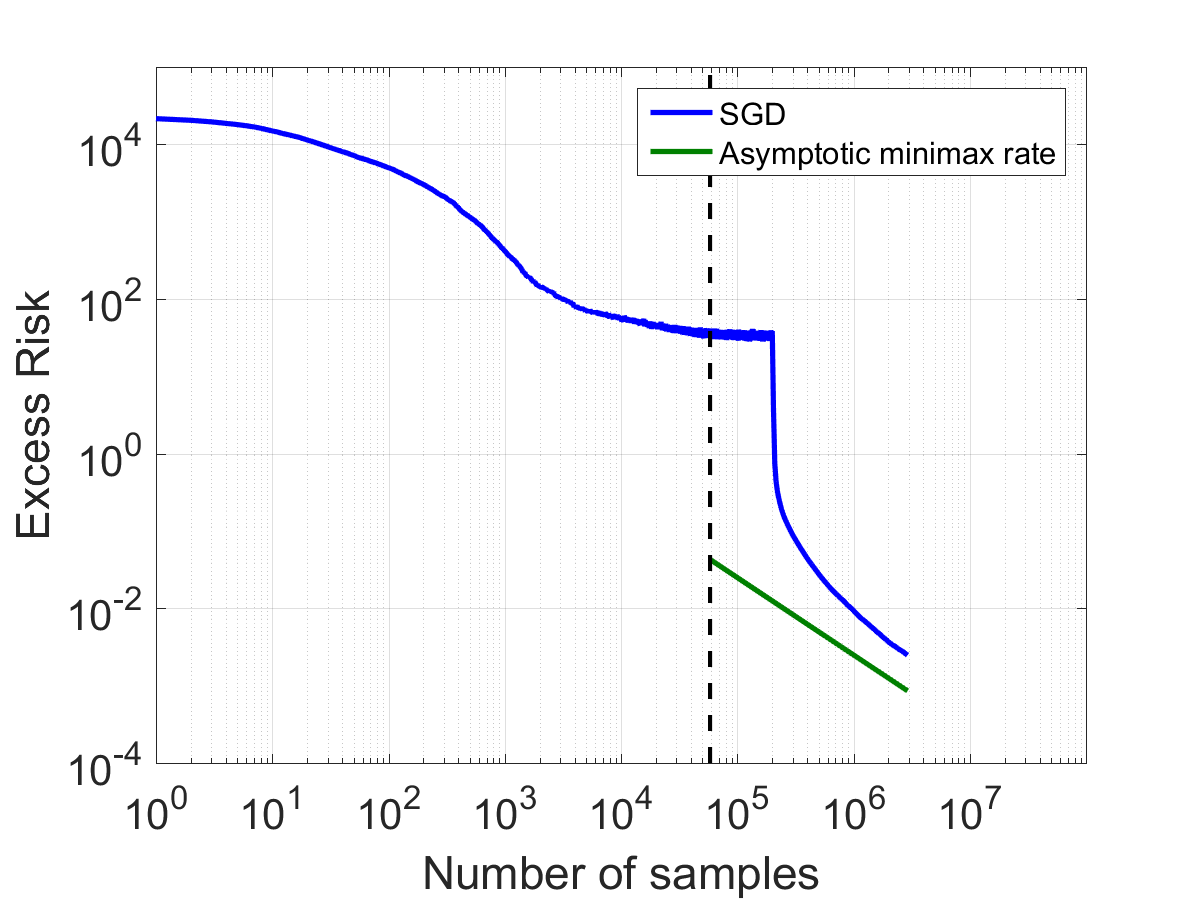
\includegraphics[width=0.49\textwidth]{figures/newer-figs/Multinomial-Total-SGD.png}}
	\subfigure[Gaussian Distribution]{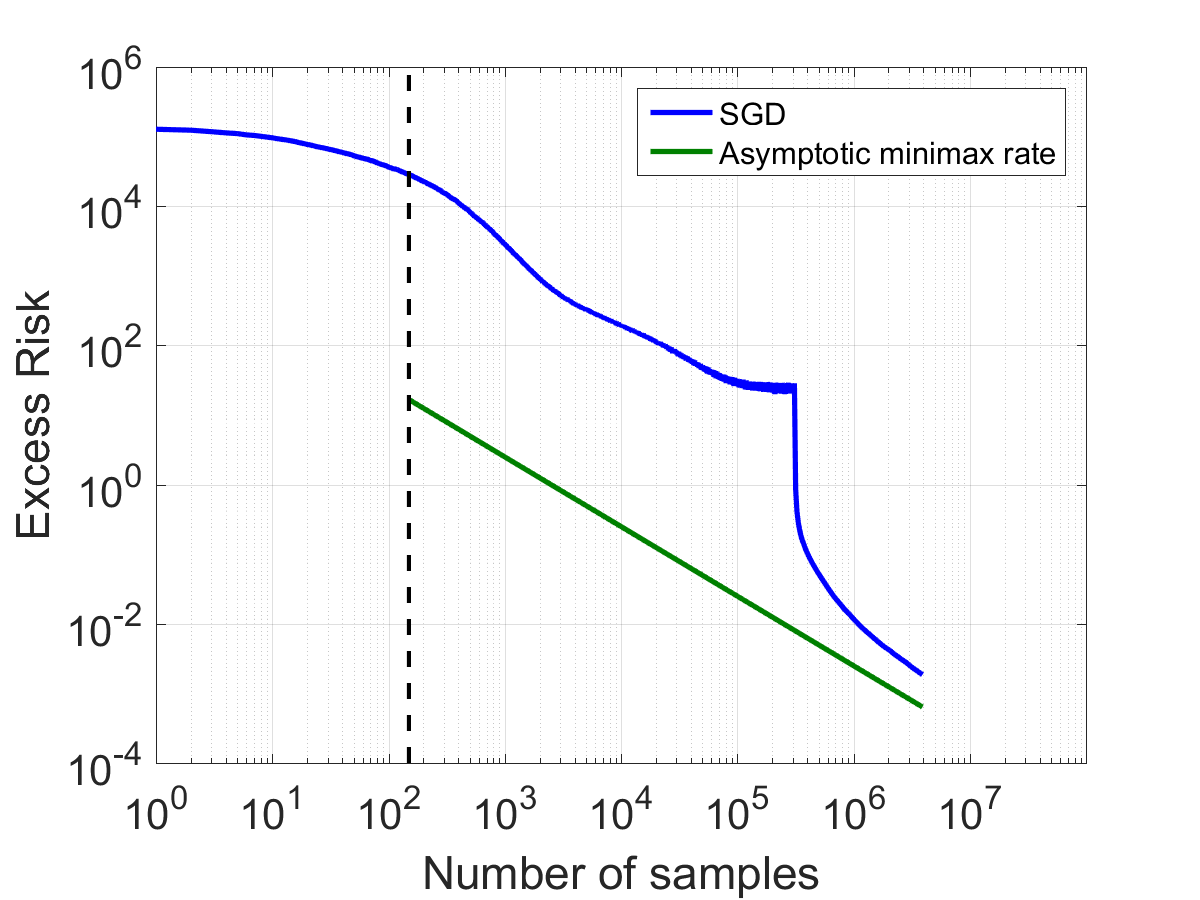
\includegraphics[width=0.49\textwidth]{figures/newer-figs/Gaussian-Total-SGD.png}}
	\vspace*{-2mm}
	\caption{Plot of total error vs number of samples for averaged
          SGD and the minimax risk (green) of $d\sigma^2/n$ for the discrete and
          Gaussian distributions with $d=50$, $\cnH\approx 10^5$ (see section~\ref{sec:exp} for
          details on the distribution). The kink in the SGD curve
          represents when the tail-averaging phase
          begins~\citep{JainKKNS16}; this point is chosen appropriately. The vertical dashed line shows the sample size at which
the empirical covariance, $\frac{1}{n}\sum_{i=1}^n \a_i\a_i\T$,
becomes full rank, which is shown at $\frac{1}{\min_i p_{i}}$ in the
discrete case and $d$ in the Gaussian case. With fewer samples than
this (i.e. before the dashed line), it is information theoretically not possible to guarantee
non-trivial risk (without further assumptions). For the Gaussian case,
note how the behavior of SGD is far from the minimax risk; it is this
behavior that one might hope to improve upon.  See the text for more discussion.
}  \vspace*{-.7cm}
\label{fig:exp} 
\end{figure}
This paper seeks to address the question: ``Can we  accelerate
stochastic approximation in a manner similar to what has been achieved
with the exact first order oracle model?''
\subsection{A thought experiment: Is Accelerating Stochastic Approximation possible?}\label{sec:exp}
Let us recollect known results in stochastic approximation for the least squares regression problem (in equation~\ref{eq:objFun}). Running $n$-steps of tail-averaged SGD~\citep{JainKKNS16} (or, streaming SVRG~\citep{FrostigGKS15}\footnote{Streaming SVRG does not function in the stochastic first order oracle model~\citep{FrostigGKS15}}) provides an output $\xhat_n$ that satisfies the following excess risk bound:
\vspace{-0.3cm}
\begin{align} \label{eq:sgd_rate}
\E{P(\xhat_n)}-P(\xs)\leq \exp(-n/\cnH) \cdot \big(P(\x_0)-P(\xs)\big) + 2\sigma^2d/n,
\end{align}

\vspace{-0.3cm}
\noindent where $\cnH$ is the condition number
of the distribution, which can be upper bounded as $L/\lamminH$,
assuming that $\|\a\|\leq L$ with probability one (refer to
section~\ref{sec:prob} for a precise definition of $\cnH$)\iffalse\footnote{technically,
  averaged SGD~\citep{JainKKNS16} contains a (lower order) factor in
  $d$ in the coefficient of the bias term.}\fi.  Under appropriate
assumptions, these are the best known rates under the stochastic first
order oracle model (see section~\ref{sec:related} for further discussion).
  A natural implication of the bound implied by averaged SGD is that with $\widetilde{\mathcal{O}}(\cnH)$ oracle
calls~\citep{JainKKNS16} (where, $\widetilde{\mathcal{O}}(\cdot)$ hides $\log$ factors in $d,\cnH$), the excess risk attains (up to
constants) the (asymptotic) minimax statistical rate. Note that the excess
risk bounds in stochastic approximation consist of two terms:
(a) {\em bias}: which represents the dependence of the generalization
error on the initial excess risk $P(\x_0)-P(\xs)$, and (b) the {\em
  variance:} which represents the dependence of the generalization
error on the noise level $\sigma^2$ in the problem.

A precise question regarding accelerating stochastic
approximation is: ``is it possible to improve the rate of decay of the
bias term, while retaining (up to constants) the statistical minimax
rate?'' The key technical challenge in answering this question is in
sharply characterizing the error accumulation of fast gradient methods
in the stochastic approximation setting. Common folklore and prior
work suggest otherwise: several efforts have attempted to 
quantify instabilities in the face of statistical or
non-statistical
errors~\citep{Paige71,Proakis74,Polyak87,Greenbaum89,RoyS90,SharmaSB98,dAspremont08,DevolderGN13,DevolderGN14,YuanYS16}.
Refer to section~\ref{sec:related} for a discussion on robustness of acceleration to error accumulation.
\begin{figure}[t]
\centering
	\subfigure[Discrete Distribution]{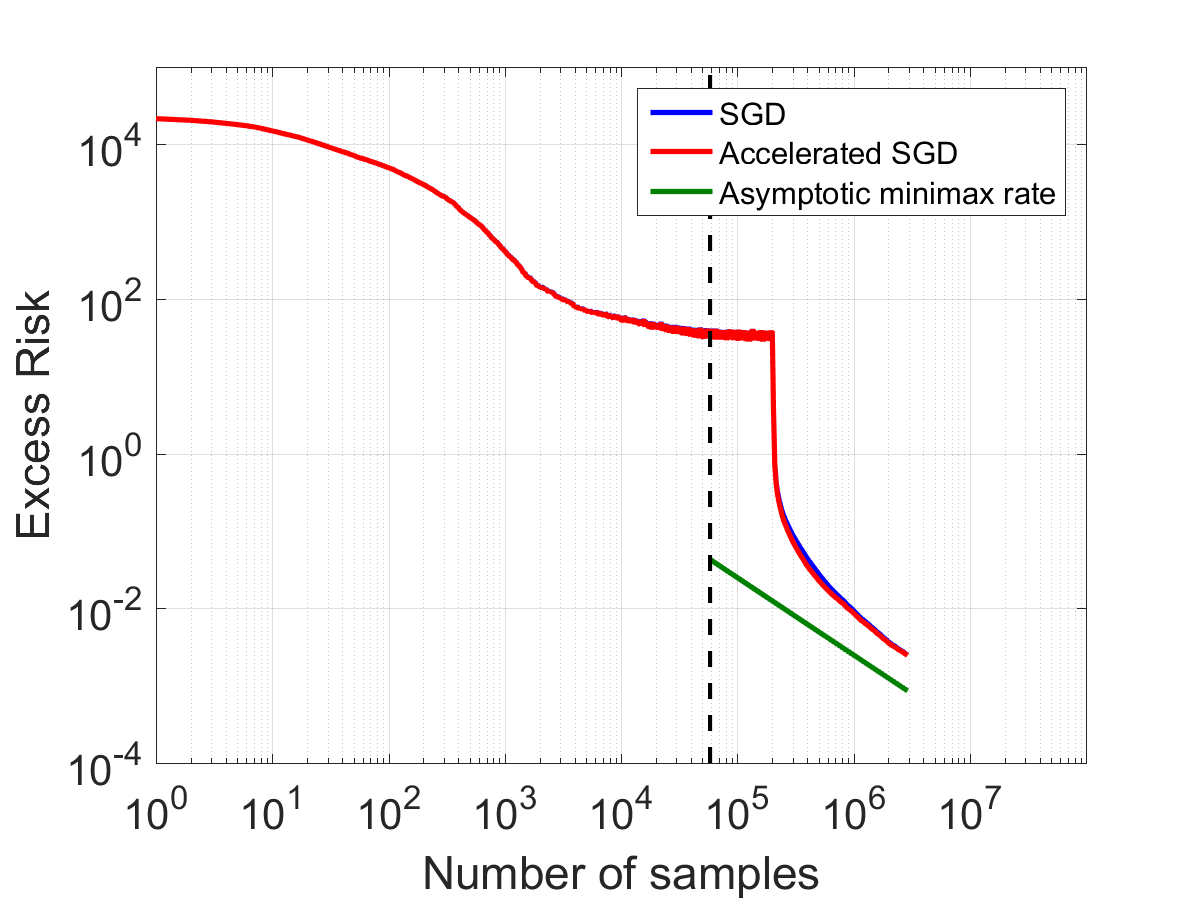
\includegraphics[width=0.49\textwidth]{figures/newer-figs/Multinomial-Total.png}}
	\subfigure[Gaussian Distribution]{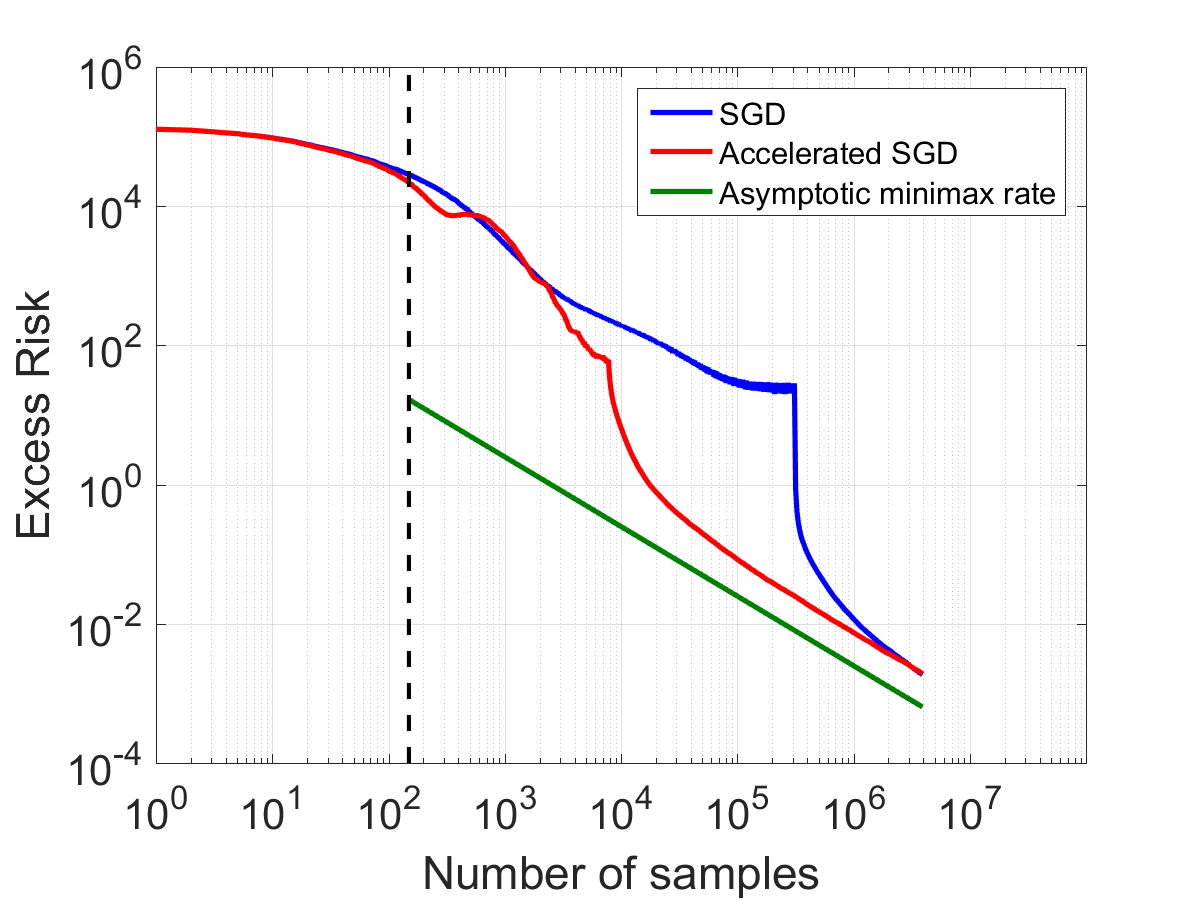
\includegraphics[width=0.49\textwidth]{figures/newer-figs/Gaussian-Total.png}}
	\vspace*{-2mm}
	\caption{Plot of total error vs number of samples for averaged
          SGD, (this paper's) accelerated SGD method and the minimax risk for the discrete and Gaussian distributions with $d=50,\cnH\approx 10^5$ (see section~\ref{sec:exp} for
          details on the distribution). For the discrete case,
          accelerated SGD mimics SGD, which nearly matches the
          minimax risk (when it becomes well defined). For the
          Gaussian case, accelerated SGD significantly improves upon
          SGD. }\vspace*{-0.8cm}\label{fig:res}
\end{figure}
Optimistically, as suggested by the gains enjoyed by accelerated methods in the exact first order oracle model, we may hope to replace the $\widetilde{\mathcal{O}}(\cnH)$ oracle calls achieved by averaged SGD to $\widetilde{\mathcal{O}}(\sqrt{\cnH})$.  We now provide a counter example, showing that such an improvement is not possible. Consider a (discrete) distribution $\D$ where the input $\a$ is the $i^{\textrm{th}}$ standard basis vector with probability $p_i$, $\forall\ i=1,2,...,d$. The covariance of $\a$ in this case is a diagonal matrix with diagonal entries $p_i$. The condition number of this distribution is $\cnH = \frac{1}{\min_i p_{i}}$. In this case, it is impossible to
make non-trivial reduction in error by observing fewer than $\cnH$ samples, since with constant probability, we would not have seen the vector corresponding to the smallest probability. 

On the other hand, consider a case where the distribution $\D$ is a
Gaussian with a large condition number $\cnH$. Matrix concentration
informs us that (with high probability and irrespective of how large $\cnH$ is) after observing
$n=\mathcal{O}(d)$ samples, the empirical covariance matrix will be a spectral approximation to the true covariance
matrix, i.e. for some constant $c>1$,
$\Cov/c \preceq \frac{1}{n}\sum_{i=1}^n \a_i\a_i\T \preceq c \Cov$.
Here, we may hope to achieve a faster convergence rate, as information
theoretically $\mathcal{O}(d)$ samples suffice to obtain a non-trivial
statistical estimate (see~\cite{HsuKZ14} for further discussion).

Figure~\ref{fig:exp} shows the behavior of SGD in these cases;
both are synthetic examples in $50-$dimensions, with a condition
number $\cnH\approx 10^5$ and noise level $\sigma^2=100$. See the figure caption for more details. 

These examples suggest that if acceleration is indeed possible, then the degree of 
improvement (say, over averaged SGD) must depend on distributional 
quantities that go beyond the condition number $\kappa$.
A natural conjecture is that this improvement must depend on 
the number of samples required to spectrally approximate 
the covariance matrix of the distribution; below this sample size it is 
not possible to obtain any non-trivial statistical estimate due 
to information theoretic reasons. This sample size is quantified by a
notion which we refer to as the {\em statistical condition number} $\cnS$ (see
section~\ref{sec:prob} for a precise definition and for further
discussion about $\cnS$). As we will see in section~\ref{sec:prob}, we have $\cnS\leq\cnH$, $\cnS$ is affine invariant, unlike $\cnH$ (i.e. $\cnS$ is invariant to linear transformations over $\a$).\vspace*{-1mm}
\begin{figure}[t]
\centering
	\subfigure[Discrete Distribution]{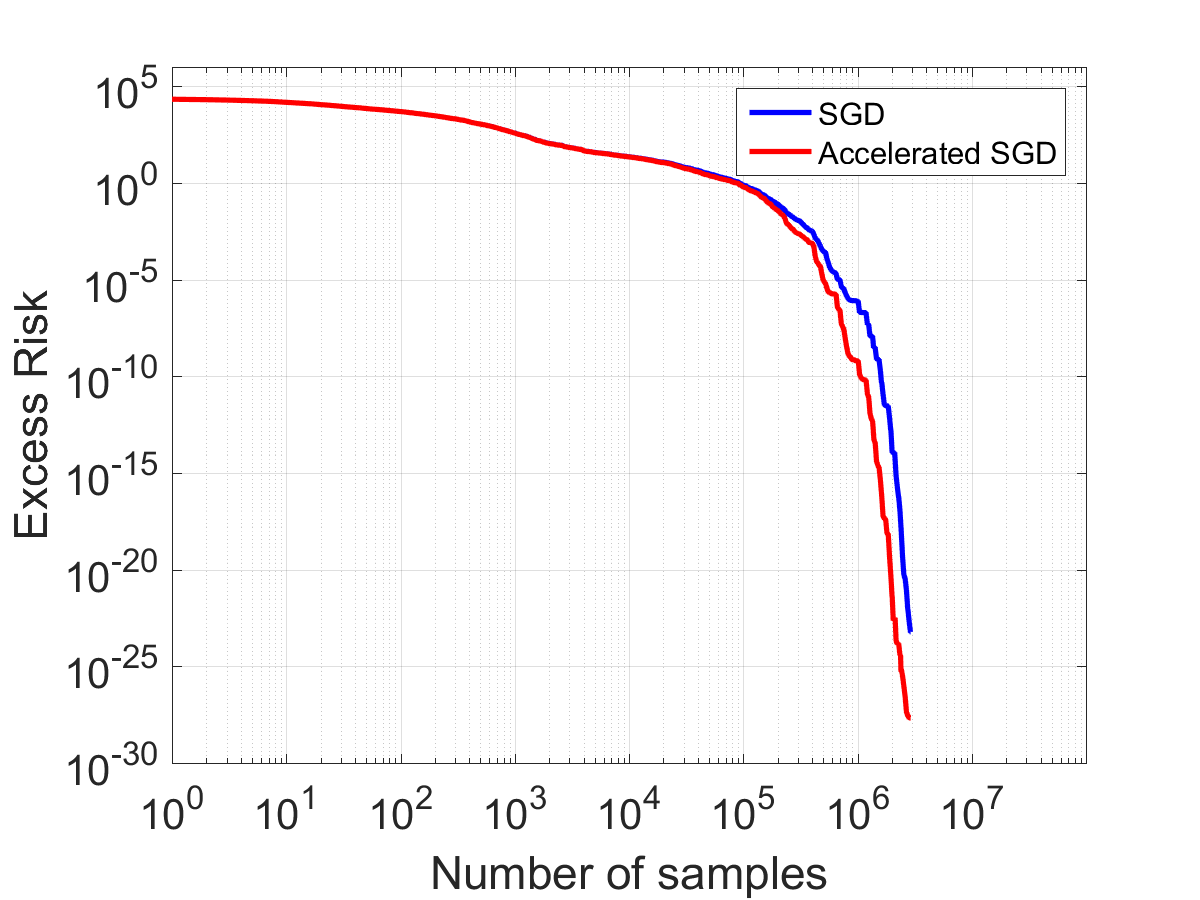
\includegraphics[width=0.49\textwidth]{figures/newer-figs/Multinomial-Bias.png}}
	\subfigure[Gaussian Distribution]{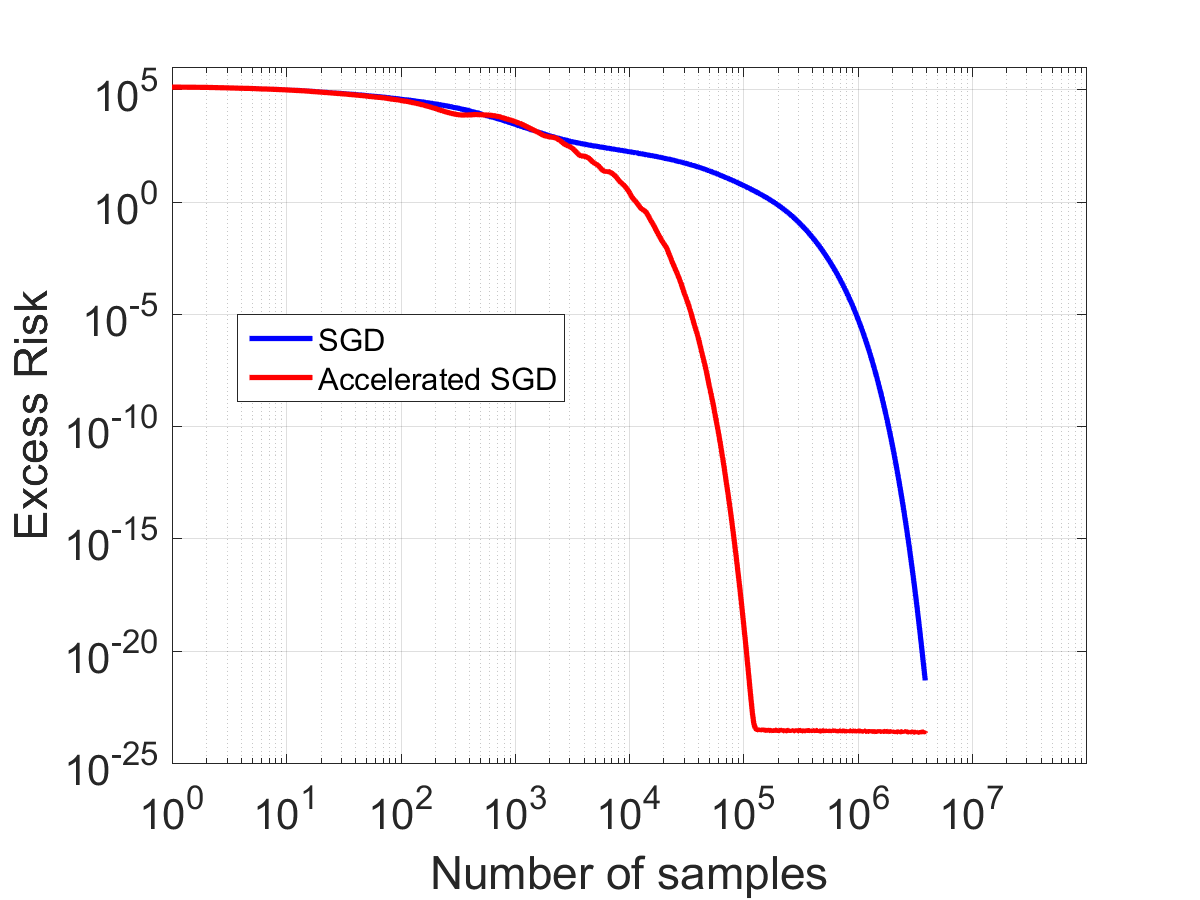
\includegraphics[width=0.49\textwidth]{figures/newer-figs/Gaussian-Bias.png}}
	\vspace*{-2mm}
\caption{Comparison of averaged SGD with this paper's accelerated SGD
  in the absence of noise ($\sigma^2=0$) for the Discrete and Gaussian
  distributions with $d=50,\cnH\approx 10^5$. Acceleration yields
  substantial gains over averaged SGD for the Gaussian case, while
  degenerating to SGD's behavior for the discrete case.
  See section~\ref{sec:exp} for discussion.}\vspace*{-0.8cm}
\label{fig:bias}
\end{figure}
\subsection{Contributions}\label{sec:res}
This paper introduces an accelerated stochastic gradient descent
scheme, which can be viewed as a stochastic variant of Nesterov's accelerated gradient method~\citep{Nesterov12}. As pointed out in Section~\ref{sec:exp}, the excess risk of this algorithm can be decomposed into two parts namely, \emph{bias} and \emph{variance}. For the stochastic approximation problem of least squares regression, this paper establishes bias contraction at a geometric rate of $\mathcal{O}(1/\sqrt{\cnH\cnS})$, improving over prior results~\citep{FrostigGKS15,JainKKNS16},\iffalse (such as averaged SGD~\citep{JainKKNS16}, streaming SVRG~\citep{FrostigGKS15}),\fi which prove a geometric rate of $\mathcal{O}(1/\cnH)$, while retaining statistical minimax rates (up to constants) for the variance. Here $\cnH$ is the condition number and $\cnS$ is the statistical condition number of the distribution, and a rate of $\mathcal{O}(1/\sqrt{\cnH\cnS})$ is an improvement over $\mathcal{O}(1/\cnH)$ since $\cnS \leq \cnH$ (see Section~\ref{sec:prob} for definitions and a short proof of $\cnS \leq \cnH$).

See Table~\ref{tab:comp} for a theoretical comparison. Figure~\ref{fig:res} provides an empirical comparison of the proposed (tail-averaged) accelerated algorithm to (tail-averaged) SGD~\citep{JainKKNS16} on our two running examples. Our result gives improvement over SGD even in the noiseless (i.e. realizable) case where $\sigma=0$; this case is equivalent to the setting where we have a distribution over a (possibly infinite) set of consistent linear equations. See Figure~\ref{fig:bias} for a comparison
on the case where $\sigma=0$.


On a more technical note, this paper introduces two new techniques in
order to analyze the proposed accelerated stochastic gradient method:
(a) the paper introduces a new potential function in order to
show faster rates of decaying the bias, and (b) the paper
provides a sharp understanding of the behavior of the
proposed accelerated stochastic gradient descent updates as a
stochastic process and utilizes this in providing a near-exact
estimate of the covariance of its iterates. This
viewpoint is critical in order to prove that the algorithm
achieves the statistical minimax rate. 

We use the operator viewpoint for analyzing stochastic
gradient methods, introduced in~\cite{DefossezB15}. This
viewpoint was also used in~\cite{DieuleveutB15,JainKKNS16}.
